\documentclass{beamer}

\usepackage[utf8x]{inputenc} 
\usepackage[slovene,english]{babel}
\usepackage{amssymb}
\usepackage{amsmath}
\usepackage{amsthm}
\usepackage{svg}
\usepackage{ulem}
\usepackage{graphicx}

\usetheme{Madrid}

\setbeamercovered{transparent=25} % pause environment is transparent

% command semitransp to make text semitransparent (actually mixes text with background color to make it appear semitransparent)
\newcommand{\semitransp}[2][25]{\color{fg!#1}#2\color{fg}}

\title{Surface simplification}
\subtitle{Project presentation}
\author{Jakob Drusany, Yon Ploj}
\institute[TDA]{Topological data analysis}
\date{\selectlanguage{slovene}\today}

\graphicspath{ {slike/} }


\begin{document}

\begin{frame}
    \titlepage
\end{frame}

\begin{frame}[t]
    \frametitle{Motivation}
    \begin{itemize}
        \item Reduce complexity
        \item Reduce measurement noise
        \item Features at various levels of resolution
        \begin{figure}
            \begin{minipage}{.5\textwidth}
                \centering
                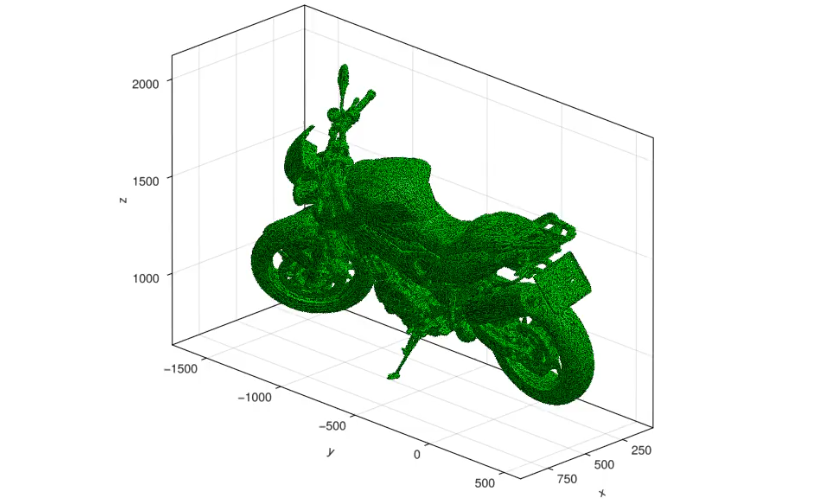
\includegraphics[width=1\textwidth]{motor_before.png}
            \end{minipage}%
            \begin{minipage}{.5\textwidth}
                \centering
                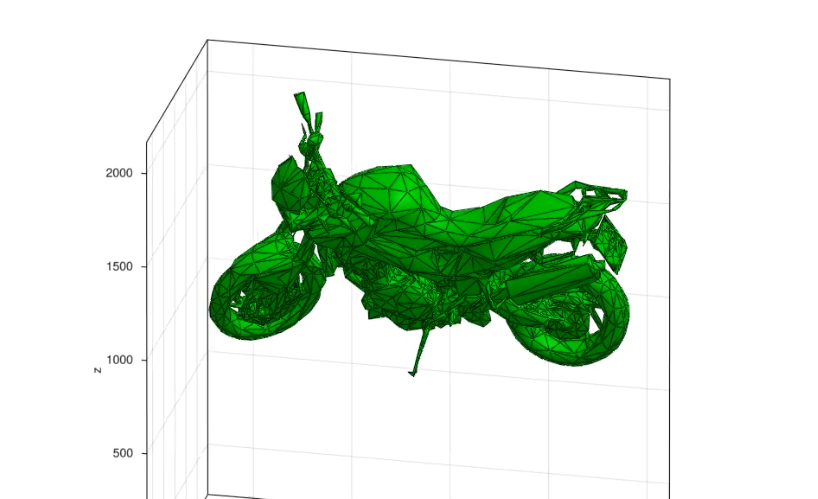
\includegraphics[width=1\textwidth]{motor_after.png}
            \end{minipage}
        \end{figure}
    \end{itemize}
\end{frame}

\begin{frame}[t]
    \frametitle{Edge contraction}
    \begin{itemize}
        \item To contract $ab$, we remove the two dark triangles and repair the hole
        by gluing their two left edges to their two right edges.
        \begin{figure}[h]
            \begin{center}
            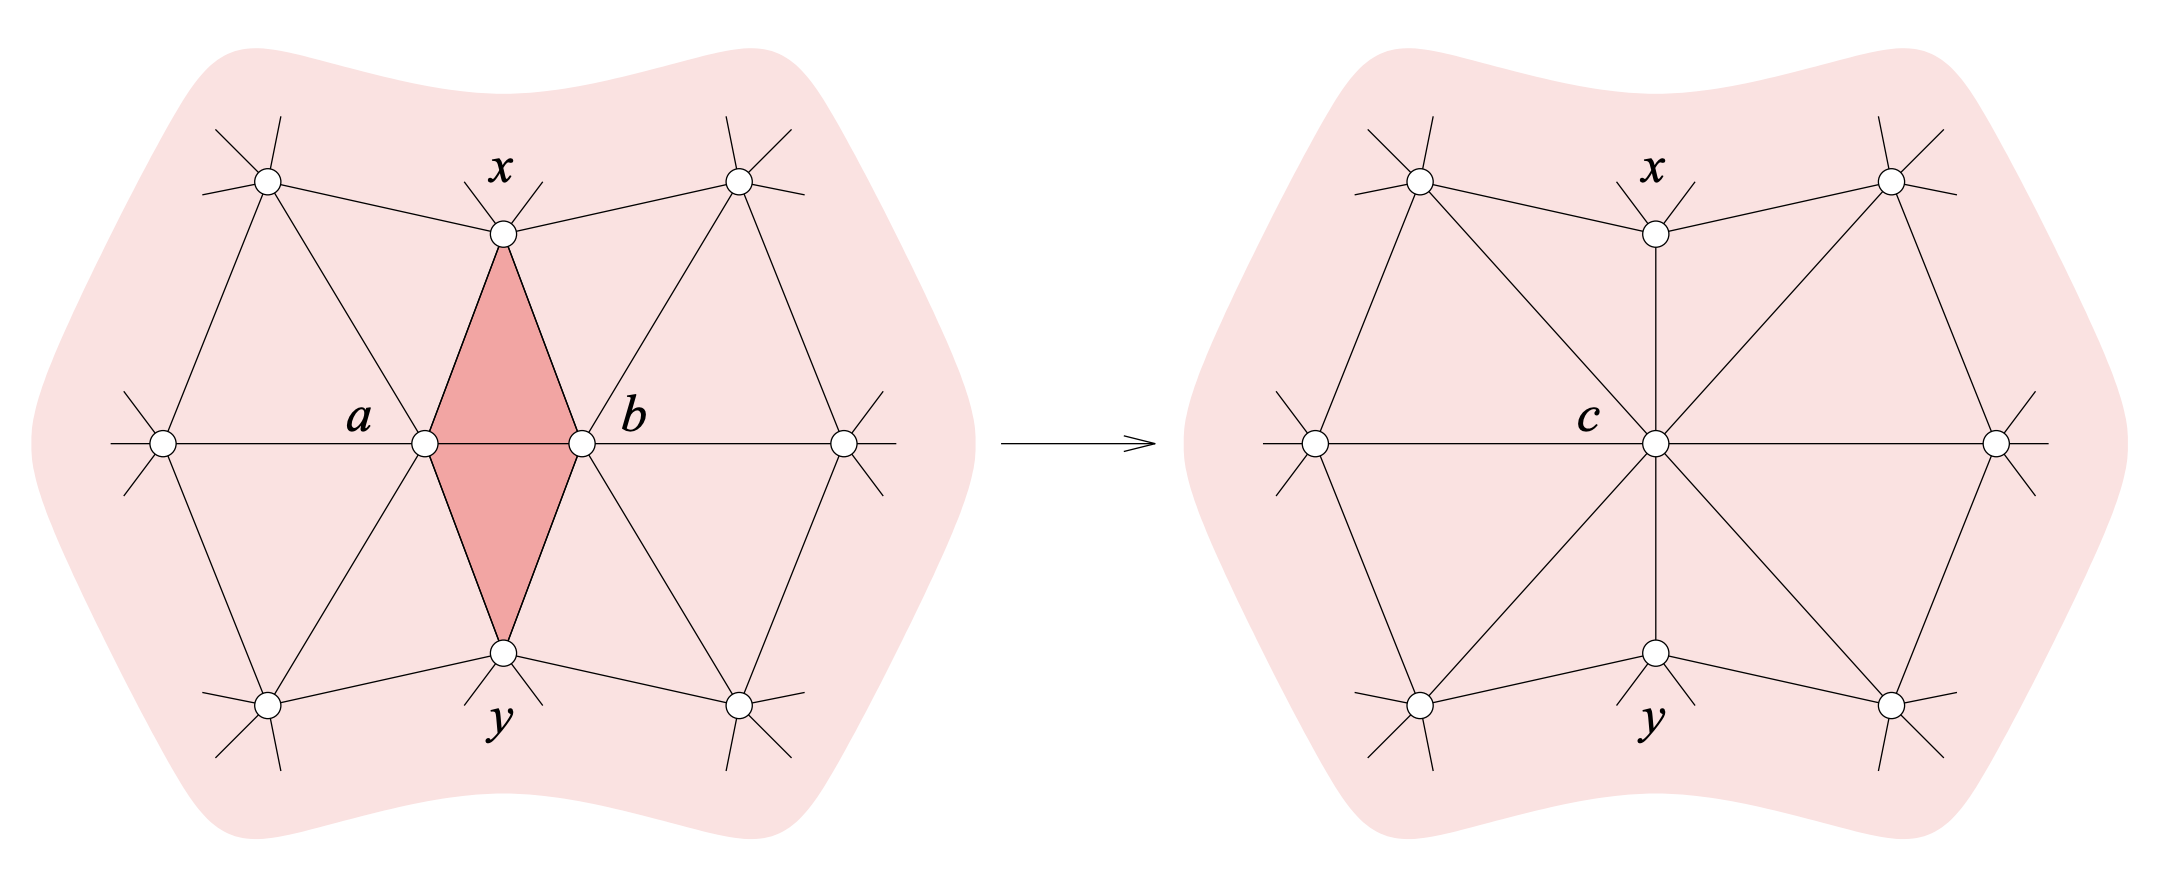
\includegraphics[width=0.8\textwidth]{edge_contract.png}
            \end{center}
        \end{figure}
        \item We want to prioritize the edges so that contractions that preserve
        the shape of the manifold are preferred
    \end{itemize}
\end{frame}
\begin{frame}[t]
    \frametitle{Chosing the point $c$}
    \begin{itemize}
    
        \item Where do we place $c$?
        \begin{figure}[h]
            \begin{center}
                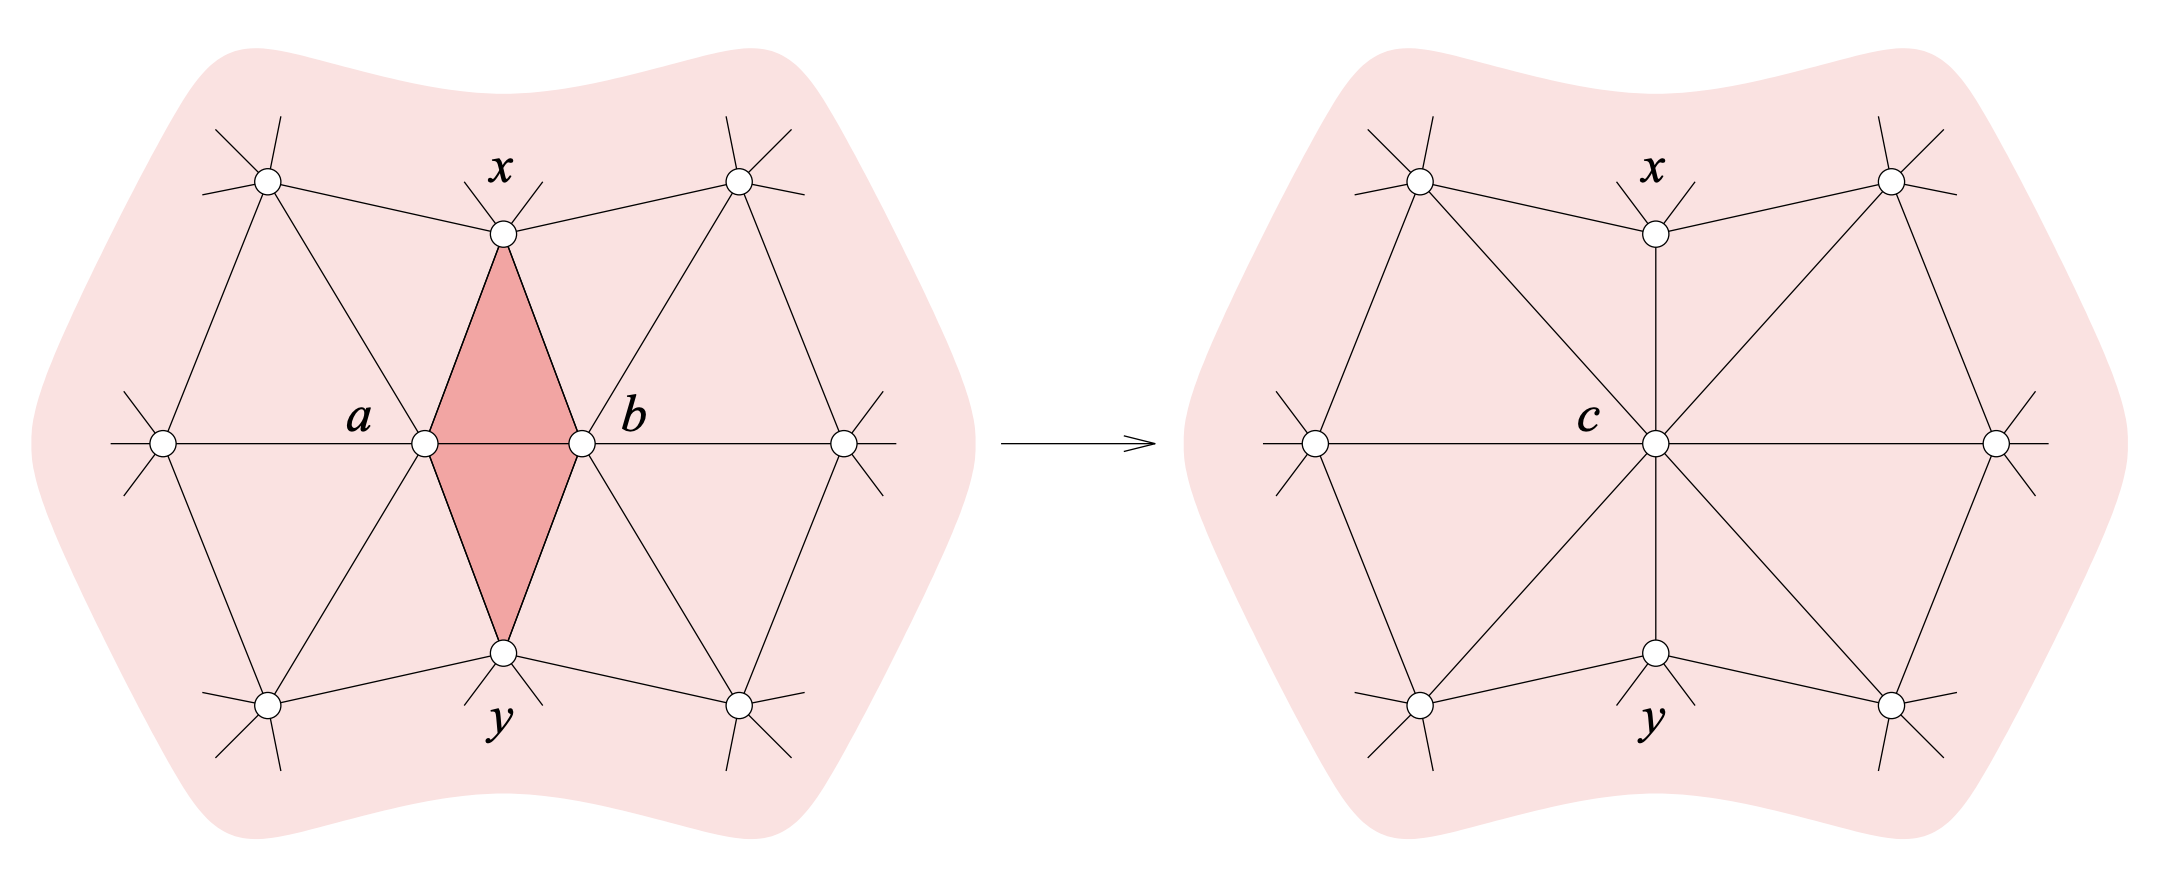
\includegraphics[width=0.7\textwidth]{edge_contract.png}
            \end{center}
        \end{figure}
        \[E_H(x) = \sum_{h_i \in H} d^2(x, h_i)\]
        \item The point $c$ has to minimize the error for a given edge $ab$
        \[Error(ab) = \min_{c\in \mathbb{R}^3} E_H(c).\]
    \end{itemize}
\end{frame}
\begin{frame}[t]
    \frametitle{Calculating the error}
    \begin{itemize}
        \item A point $x$ can be represented as a vector $x^T = (x'^T, 1)$  
        \item A plane $y \in \mathbb{R}^3, <y, u'> = -\delta$ can be represented
        as a vector $u^T = (u'^T, \delta)$
        \item We use this to express the sum of squared distances
        from a set of planes in matrix form $H$
        \begin{align*}
            E_H(x) &= \sum_{h_i \in H} d^2(x, h_i)\\
                   &=\sum_{h_i \in H} (x^T \cdot u_i) (u_i^T \cdot x)\\
                   &= x^T \cdot \left( \sum_{h_i \in H} u_i \cdot u_i^T \right) \cdot x
        \end{align*}
    \end{itemize}
\end{frame}
\begin{frame}[t]
    \frametitle{$Q$ matrix}
    \begin{itemize}
        \item We can define the $Q$ matrix as \[Q = \sum_{h_i \in H} u_i \cdot u_i^T\]
        so the following holds: $E_H(x) = x^T \cdot Q \cdot x$
        \item The $Q$ matrix is a symmetric, four-by-four matrix we refer to as the fundamental quadric of
        the map $E_H$
        \item $Q_a$ represents the matrix of all planes of which the triangles
        contain the vertex $a$
        \item $Q_{ab}$ represents the matrix of all planes of which the triangles
        contain the edge $ab$
        \item $Q_{abc}$ represents the matrix of the plane of $abc$
    \end{itemize}
\end{frame}
\begin{frame}[t]
    \frametitle{Computing the minimum}
    \begin{itemize}
        \item We can find the minimum simply by solving the equation
        \[
            Q_{ab}[1:3, :] \cdot x = 0
        \]
        \item We have to find a solution where $x[4]$ is not 0
    \end{itemize}
\end{frame}
\begin{frame}[t]
    \frametitle{Implementation problems 1}
    \begin{itemize}
        \item The triangles are not connected
            \begin{figure}[h]
                \begin{center}
                    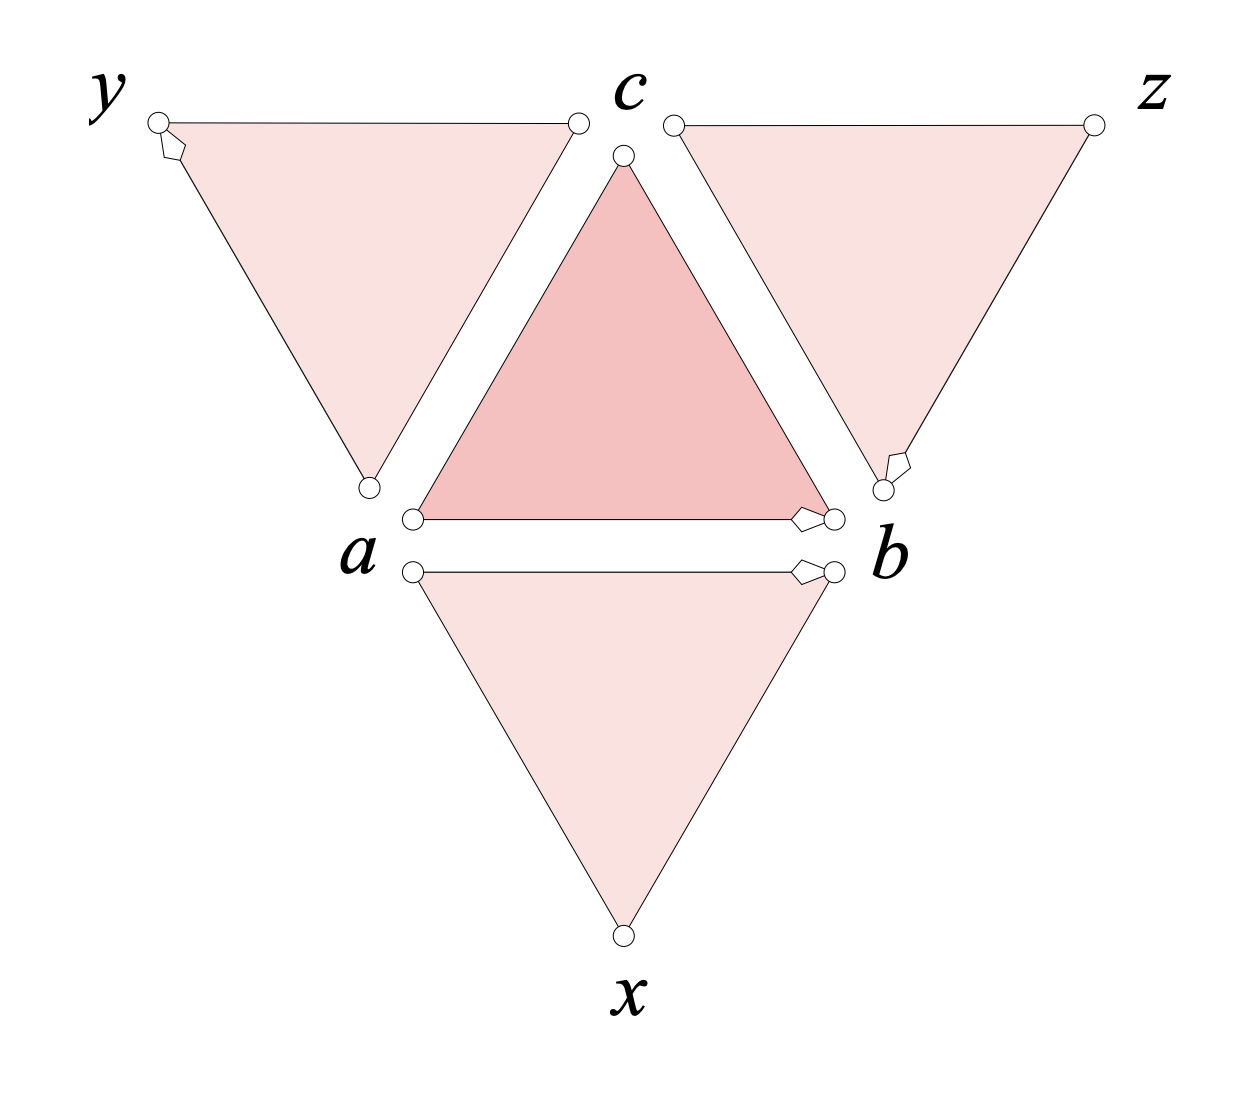
\includegraphics[width=0.4\textwidth]{triangles.png}
                \end{center}
            \end{figure}
    \end{itemize}
\end{frame}
\begin{frame}[t]
    \frametitle{Implementation problems 2}
    \begin{itemize}
        \item The mesh is not a manifold
            \begin{figure}[h]
                \begin{center}
                    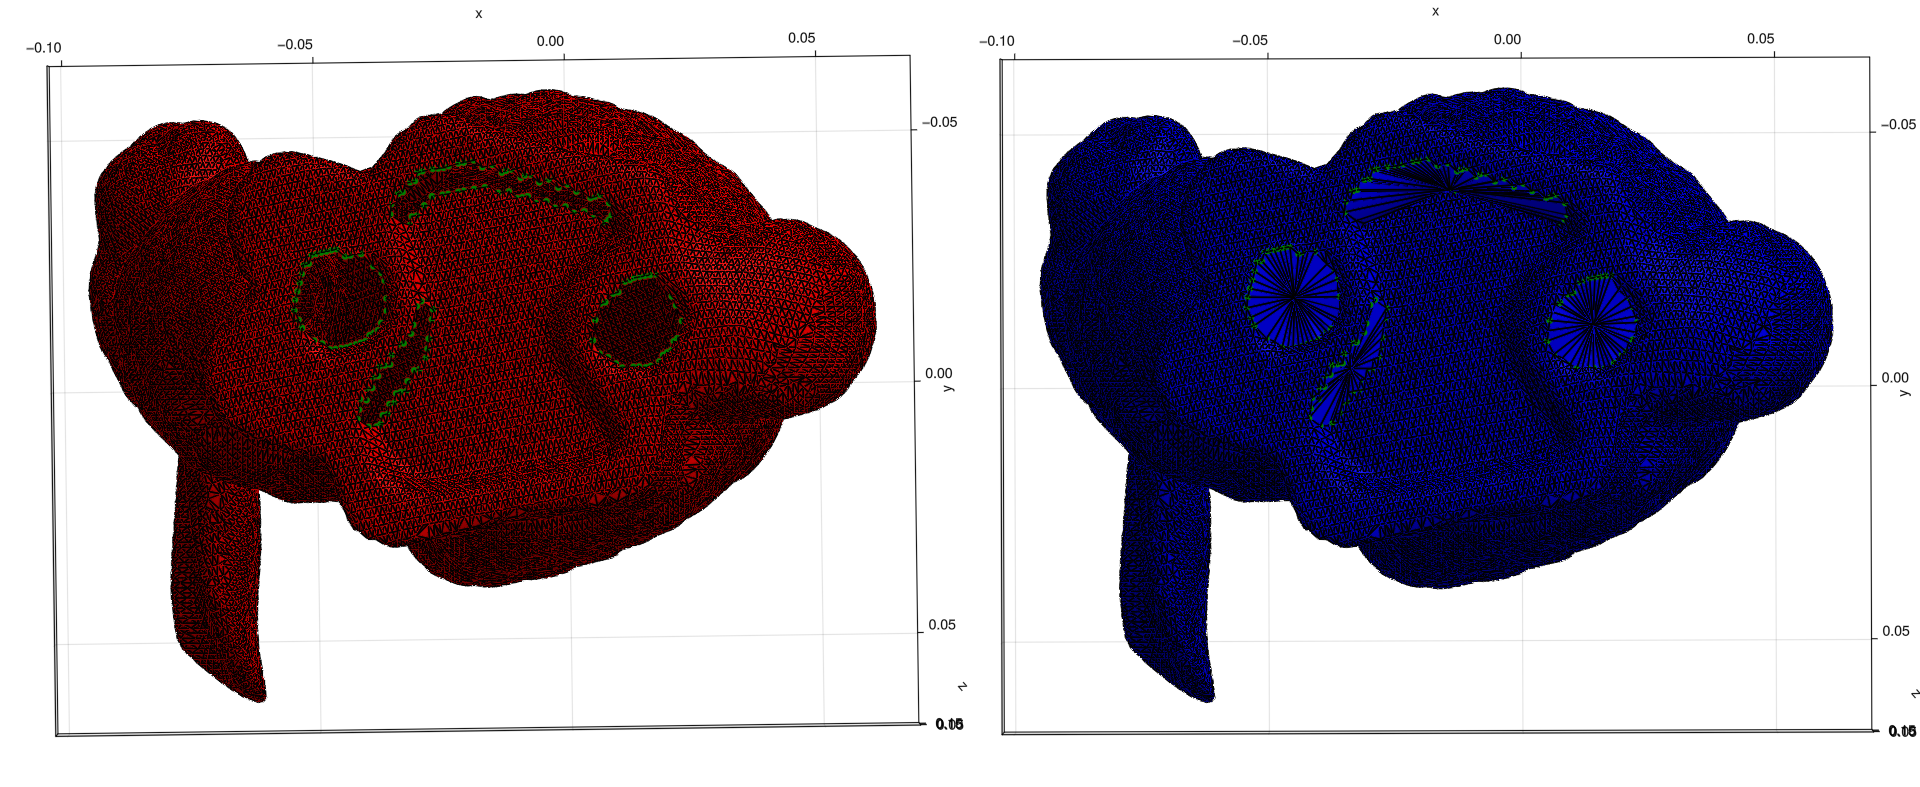
\includegraphics[width=0.9\textwidth]{butthole.png}
                \end{center}
            \end{figure}
    \end{itemize}
\end{frame}

\end{document}